%%%%%%%%%%%%%%%%%%%%%%%%%%%%%%%%%%%%%%%%%%%%%%%%%%%%%%%%%%%%%%%%%%%%%%%%%%%%%%%%
% VHDL Entity Diagram Example
% v.01 16/05/2020
%
% entity_example.tex
% (c) Copyright 2020 - Will Frank
%
% This work may be distributed and/or modified under the conditions of the LaTeX
% Project Public License, either version 1.3 of this license or (at your option)
% any later version.
%
% The latest version of this license is in:
%     http://www.latex-project.org/lppl.txt
% and version 1.3 or later is part of all distributions of LaTeX version
% 2005/12/01 or later.
%
% This work has the LPPL maintenance status `maintained'.
%
% The Current Maintainer of this work is Will Frank.
%
% This work consists of the file(s): entity_example.tex.
%%%%%%%%%%%%%%%%%%%%%%%%%%%%%%%%%%%%%%%%%%%%%%%%%%%%%%%%%%%%%%%%%%%%%%%%%%%%%%%%

\documentclass{standalone}
\usepackage{tikz}
\usetikzlibrary{matrix, positioning, arrows, decorations.markings}

\newlength{\myheight}
\setlength{\myheight}{2.5cm}

% Configure TikZ style
\tikzset
{
    labels/.style={font=\sffamily\scriptsize},
    circuit/.style={draw,minimum width=2cm,minimum height=\myheight,very thick,
    inner sep=1mm,outer sep=0pt,cap=round,font=\sffamily\bfseries},
    decoration={markings,mark=at position 0.5 with
    {\node[font=\footnotesize] {/};}}
}

\begin{document}
    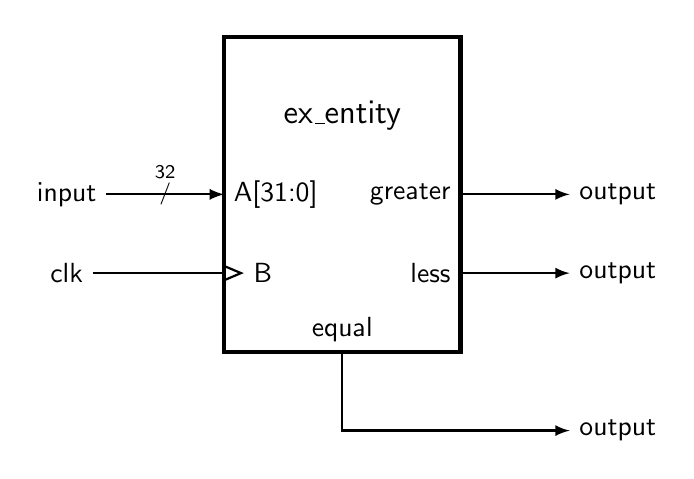
\begin{tikzpicture}[font=\sffamily,>=latex]

    % Entity black box
    \path[draw,ultra thick] (0,0) node (A){} --(0,4) node (B){}-- (3,4) node
    (C){} --(3,0) node (D){}--cycle;

    % Input/output port(s) node(s) and label(s)
    \node (cent) at (1.5,3){\large ex\_entity};
    \node[right] (AB1) at (0,2) {A[31:0]};
    \node[right] (AB2) at (0.25,1) {B};
    \node[left] (CD1) at (3,1) {less};
    \node[left] (CD2) at (3,2) {greater};
    \node[above] (AD) at (1.5,0) {equal};

    % Wire(s) label(s)
    \node (A1) at (-2,2) {input};
    \node (A2) at (-2,1) {clk};
    \node (C1) at (5,1) {output};
    \node (C2) at (5,2) {output};
    \node (D1) at (5,-1) {output};

    % Wire(s) arrow(s)
    \draw[->, thick, postaction={decorate}] (A1)-- node[above=2pt] {\scriptsize
    32}(AB1);
    \draw[-open triangle 45, thick] (A2)--(AB2);
    \draw[->, thick] (CD1)--(C1);
    \draw[->, thick] (CD2)--(C2);
    \draw[->, thick] (AD)|-(D1);

    \end{tikzpicture}
\end{document}
